\documentclass[a4paper, 12pt, twoside]{article}
\usepackage[T2A,T1]{fontenc}
\usepackage[utf8]{inputenc}
\usepackage[english, russian]{babel}
\usepackage{graphicx}
\usepackage[hcentering, bindingoffset = 10mm, right = 15 mm, left = 15 mm, top=20mm, bottom = 20 mm]{geometry}
\usepackage{multirow}
\usepackage{ gensymb }
\usepackage{lipsum}
\usepackage{amsmath, amstext}
\usepackage{siunitx}
\usepackage{subcaption}
\usepackage{wrapfig}
\usepackage{adjustbox}
\usepackage{enumerate, indentfirst, float}
\usepackage{capt-of, svg}
\usepackage{ctable}

\newcommand*{\hm}[1]{#1\nobreak\discretionary{} 
	{\hbox{$\mathsurround=0pt #1$}}{}}
\usepackage{cmap} % Улучшенный поиск русских слов в полученном pdf-файле

\usepackage{pscyr} % Нормальные шрифты
\usepackage[normalem]{ulem} % для подчёркиваний uline
\ULdepth = 0.16em

\usepackage{fancyhdr} %Колонтикулы
\pagestyle{fancy}
\lhead{
\includegraphics[width = 10 mm]{logo.jpg} Лабораторная работа № 4.2.1}
\rhead{\textit{5 апреля 2018 г.}}

\newenvironment{bottompar}{\par\vspace*{\fill}}{\clearpage}

\begin{document}
	\begin{titlepage}
		
		\newcommand{\HRule}{\rule{\linewidth}{0.7mm}} % Defines a new command for the horizontal lines, change thickness here
		
		\center % Center everything on the page
		
		%----------------------------------------------------------------------------------------
		%	HEADING SECTIONS
		%----------------------------------------------------------------------------------------
		
		\textsc{\LARGE Московский Физико-Технический Институт}\\[1,5cm] % Name of your university/college
		\textsc{\Large Кафедра общей физики}\\[0.5cm] % Major heading such as course name
		\textsc{\large Лабораторная работа \textnumero  4.2.1}\\[0.5cm] % Minor heading such as course title
		
		%----------------------------------------------------------------------------------------
		%	TITLE SECTION
		%----------------------------------------------------------------------------------------
		
		\HRule
		\\[0.4cm]
		{ \huge \bfseries Кольца Ньютона}
		\\[0.2cm] % Title of your document
		\HRule
		\\[1.5cm]
		
		
		
		%----------------------------------------------------------------------------------------
		%	AUTHOR SECTION
		%----------------------------------------------------------------------------------------
		
		\begin{minipage}{0.4\textwidth}
			\begin{flushleft} \large
				\textbf{Автор:}\\
				Глеб Уваркин \\
				615 группа
			\end{flushleft}
		\end{minipage}
		~
		\begin{minipage}{0.4\textwidth}
			\begin{flushright} \large
				\textbf {Преподаватель:} \\
				Клёнов Сергей Львович % Supervisor's Name
			\end{flushright}
		\end{minipage}
		
		\begin{bottompar}
			\begin{center}
				
\includegraphics[width = 80 mm]{logo.jpg}
			\end{center}
			{\large 5 апреля 2018 г.}
			
		\end{bottompar}
		\vfill % Fill the rest of the page with whitespace
		
	\end{titlepage}
	
	{\Large \uline { \textbf  {Цель работы:}}}
	
	\vspace{2mm}
	Познакомиться с явлением интерференции в тонких плёнках (полосы равной толщины) на примере колец Ньютона и с методикой интерференционных измерений кривизны стеклянной поверхности
	\vspace{\baselineskip}
	
	{\Large \uline { \textbf  {В работе используются:}}}
	
	\vspace{2mm}
	
	Измерительный микроскоп с опак-иллюминатором; плосковыпуклая линза; пластинка из чёрного стекла; ртутная лампа ДРШ; щель; линзы; призма прямого зрения; объектная шкала.
	
	\section{Теоретические сведения.}
	
	В опыте колец Ньютона наблюдается интерференция волн, отражённых от границ тонкой воздушной прослойки, образованной сферической поверхностью линзы и плоской стеклянной пластиной. Схема опыта показана на рис \ref{img1}.
	
	\begin{minipage}{0.49\linewidth}
		\begin{figure}[H]
			\centering
			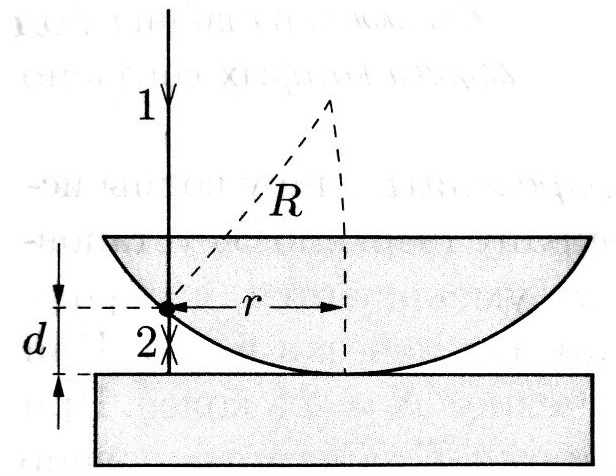
\includegraphics[width =  0.8\textwidth]{img1}
			\caption{Схема наблюдения колец Ньютона.}
			\label{img1}
		\end{figure}
	\end{minipage}
	~
	\begin{minipage}{0.49\linewidth}
		Для точки на сферической поверхности, находящейся на расстоянии $r$ от оси системы, имеем $r^2 = R^2 - (R - d)^2 = 2Rd - d^2$, где $R$ - радиус кривизны сферической поверхности. При $R \gg d$ получим $d = r^2/2R$. С учётом изменения фазы на $\pi$ при отражении волны от оптически более плотной среды (на границе воздух -- стекло) получим оптическую разность хода интерферирующих лучей: $$\Delta = 2d + \dfrac{\lambda}{2}.$$
		Условие интерференционного минимума $\Delta = (2m + 1)\frac{\lambda}{2}~(m = 0, 1, 2, ...)$, откуда получаем для радиусов тёмных колец
	\end{minipage}\\
	
	\begin{equation}
	r'_m = \sqrt{m\lambda R}.
	\label{eq1}
	\end{equation}
	
	Аналогично для радиусов $r_m$ светлых колец 
	
	\begin{equation}
	r'_m = \sqrt{(2m - 1) \lambda R/2}.
	\label{eq2}
	\end{equation}
	
	\paragraph*{Наблюдение биений.} При освещении системы светом, содержащим две спектральные компоненты (с длинами $\lambda_1$ и $\lambda_2$, $\lambda_2 < \lambda_1$), наблюдается характерная картина биений: чёткость интерференционных колец периодически изменяется. Это объясняется наложением двух систем интерференционных колец. Размытые кольца получаются при наложении светлых колец одной картины на тёмные кольца другой.
	
	Рассчитаем период возникающих биений. Пусть в промежутке между двумя центрами соседних чётких участков укладывается $\Delta m$ колец для спектральной линии с длиной волны $\lambda_1$. Тогда в этом промежутке должно располагаться $(\Delta m + 1)$ колец для спектральной линии с длиной волны $\lambda_2$. Найдём условие наложения максимумов:
	\begin{equation}
	\Delta m \lambda_1 = (\Delta m + 1)\lambda_2 \Longrightarrow \Delta \lambda = \dfrac{\lambda_2}{\Delta m}
	\label{eq3}
	\end{equation}
	
	\section{Экспериментальная установка.}
	
	\begin{figure}[H]
		\centering
		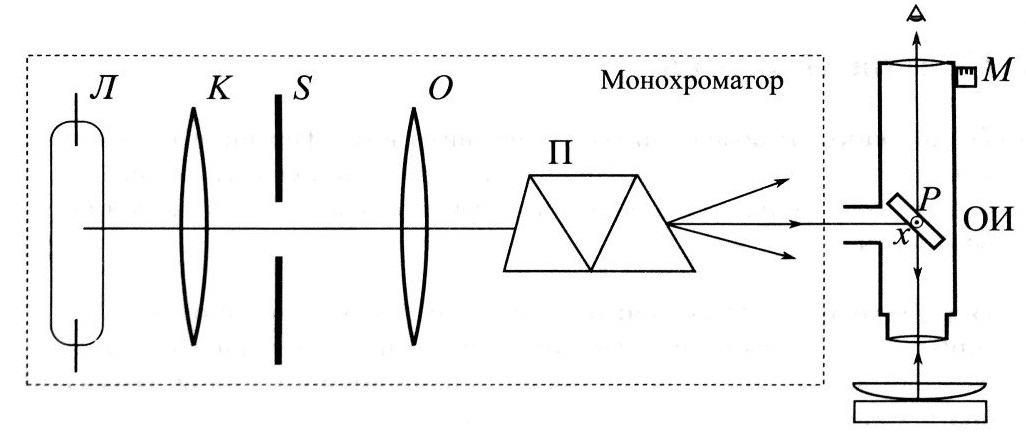
\includegraphics[width =  0.8\textwidth]{img2}
		\caption{Схема установки для наблюдения колец Ньютона.}
		\label{img2}
	\end{figure}

	Схема экспериментальной установки приведена на рис. \ref{img2}. Источником света служит ртутная лампа, находящаяся в защитном кожухе. Для получения монохроматического света применяется призменный монохроматор, состоящий из конденсора $K$, коллиматора (щель $S$ и объектив $O$) и призмы прямого зрения $\Pi$. Свет от монохроматора попадает на опак-иллюминатор (ОИ), расположенный между окуляром и объективом микроскопа -- специальное устройство для освещения объекта при работе в отражённом свете. Внутри опак-иллюминатора находится полупрозрачная пластинка $P$, наклоненная под углом $45\degree$ к оптической оси микроскопа.
	
	Оптическая схема монохроматора позволяет получить в плоскости входного окна опак-иллюминатора достаточно хорошо разделённые линии спектра ртутной лампы. Изображение щели $S$ фокусируется на поверхность линзы объективом микроскопа, и в том же месте находится плоскость наблюдения микроскопа, т.е. точка источника и точка наблюдения интерференции совпадают. Картина интерференции как и в случае расположения пластинки сверху, так и в данном случае не зависит от коэффициента преломления линзы и определяется величиной зазора между нижней поверхностью линзы и стеклянной пластинкой.
	
	\section{Ход работы.}
	
	\subsection{Измерение диаметров колец.}
	
	Снимем показания окулярной шкалы и микрометрического винта для тёмных и светлых колец (m -- номер кольца). Используем яркую зеленую линию ртути ($\lambda = 546~\text{нм}$). Результаты занесём в таблицу \ref{t1}.
	
	\begin{table}[H]
		\centering
		\caption{К определению диаметров колец.}
		\label{t1}
		\resizebox{\textwidth}{!}{
		\begin{tabular}{c|c|c|c|c|c|c|cc|c|c|c|c|c|c} \toprule
			m                            & -6   & -5   & -4   & -3   & -2   & -1   & -0        & +0        & 1    & 2    & 3    & 4    & 5    & 6    \\ \midrule
			$x_\text{тёмн},~\text{дел}$  & 1.46 & 1.62 & 1.83 & 2.05 & 2.31 & 2.64 & 3.14      & 3.89      & 4.36 & 4.73 & 5.01 & 5.23 & 5.40 & 5.59 \\ \midrule
			$x_\text{светл},~\text{дел}$ & 1.54 & 1.73 & 1.95 & 2.19 & 2.49 & 2.92 & \multicolumn{2}{c|}{-} & 4.13 & 4.51 & 4.90 & 5.11 & 5.32 & 5.50 \\ \bottomrule
		\end{tabular}
	}
	\end{table}
	
	
	\newpage
	\subsection{Наблюдение <<биений>>.}
	Получим картину <<биений>> и просчитаем количество тёмных полос $\Delta m$ от центра одной чёткой системы полос до центра соседней чёткой системы. Получаем, что $$\Delta m = 17$$.
	
	\subsection{Калибровка окулярной шкалы.}
	
	Определим цену деления окулярной шкалы с помощью калиброванной объектной шкалы. Объектная шкала размером 1 мм разбита на 100 делений.
	
	Получаем, что 
	$$7~\text{дел.ок.шк} = 69~\text{дел.об.шк}\cdot \dfrac{1~\text{мм}}{100~\text{дел}}$$
	
	

	\section{Обработка результатов.}
	\begin{enumerate}
		\item 	Рассчитаем цену деления окулярной шкалы:
			\begin{center}
				\fbox{$1~\text{дел.ок.шк} \simeq 0.1 ~ \text{мм}$}
			\end{center}
		
			Погрешность этого измерения составляет $0.01~\text{мм}$.
			
		\item  По результатам наблюдения <<биений рассчитаем>> разность длин волн для жёлтой и зелёной линии Hg с помощью формулы \eqref{eq3}. Результаты занесём в таблицу \ref{t2}.
		
		\begin{table}[H]
			\centering
			\caption{К определению $\lambda$ желтой линии.}
			\label{t2}
			\begin{tabular}{c|c|c} \toprule
				$\Delta \lambda,~\text{нм}$ & $\lambda_\text{жёлт}^{\text{пр}},~\text{нм}$ & $\lambda_\text{жёлт}^{\text{теор}},~\text{нм}$ \\ \midrule
				32                          & 578                                          & 577 -- 579     \\ \bottomrule                               
			\end{tabular}
		\end{table}
		
		\item 	Рассчитаем радиусы тёмных и светлых колец, используя таблицу \ref{t1} и результат калибровки окулярной шкалы. Построим графики зависимостей $r_m^2$ и $(r'_m)^2$ от номера m кольца. Все необходимые данные занесём в таблицу \ref{t3}.
		
		Подсчёт погрешностей:
		
		$$r^2 = \left ( \dfrac{x(m) - x(-m)}{2} \right )^2,~~m = 1, 2, \cdots, 6$$
		
		$$\sigma_{r^2} = \sqrt{\left (\frac{\partial (r^2)}{\partial x_m}\cdot \sigma_{x_m} \right )^2 + \left (\frac{\partial (r^2)}{\partial x_{-m}}\cdot \sigma_{x_{-m}} \right )^2} = \sqrt{2\left (\frac{x_m - x_{-m}}{2}\right ) \cdot \sigma_{x_m}^2} = \dfrac{d\cdot \sigma_x}{\sqrt{2}}$$
		
		\begin{table}[H]
			\centering
			\caption{Определение $r^2$.}
			\label{t3}
			\begin{tabular}{c|c|c|c|c} \toprule
				m & $d_\text{темн}, ~\text{мм}$ & $d_\text{светл}, ~\text{мм}$ & $r'^2,~\text{мкм}$ & $r^2,~\text{мкм}$ \\ \midrule
				1 & 0.17                        & 0.12                         & $7.4 ~\pm$ 0.1      & $3.7~ \pm$ 0.1     \\
				2 & 0.24                        & 0.20                         & $14.6~\pm$ 0.2      & $10.2 ~\pm$ 0.1    \\
				3 & 0.29                        & 0.27                         & $21.9 ~\pm$ 0.2     & $18.4 ~\pm$ 0.2    \\
				4 & 0.34                        & 0.32                         & $28.9~\pm$ 0.2      & $24.9 ~\pm$ 0.2    \\
				5 & 0.38                        & 0.36                         & $35.7 ~\pm$ 0.3     & $32.2 ~\pm $ 0.3   \\
				6 & 0.41                        & 0.39                         & $42.6~ \pm$ 0.3     & $39.2 ~\pm$ 0.3  \\ \bottomrule 
			\end{tabular}
		\end{table}
	
		\begin{figure}[H]
			\centering
			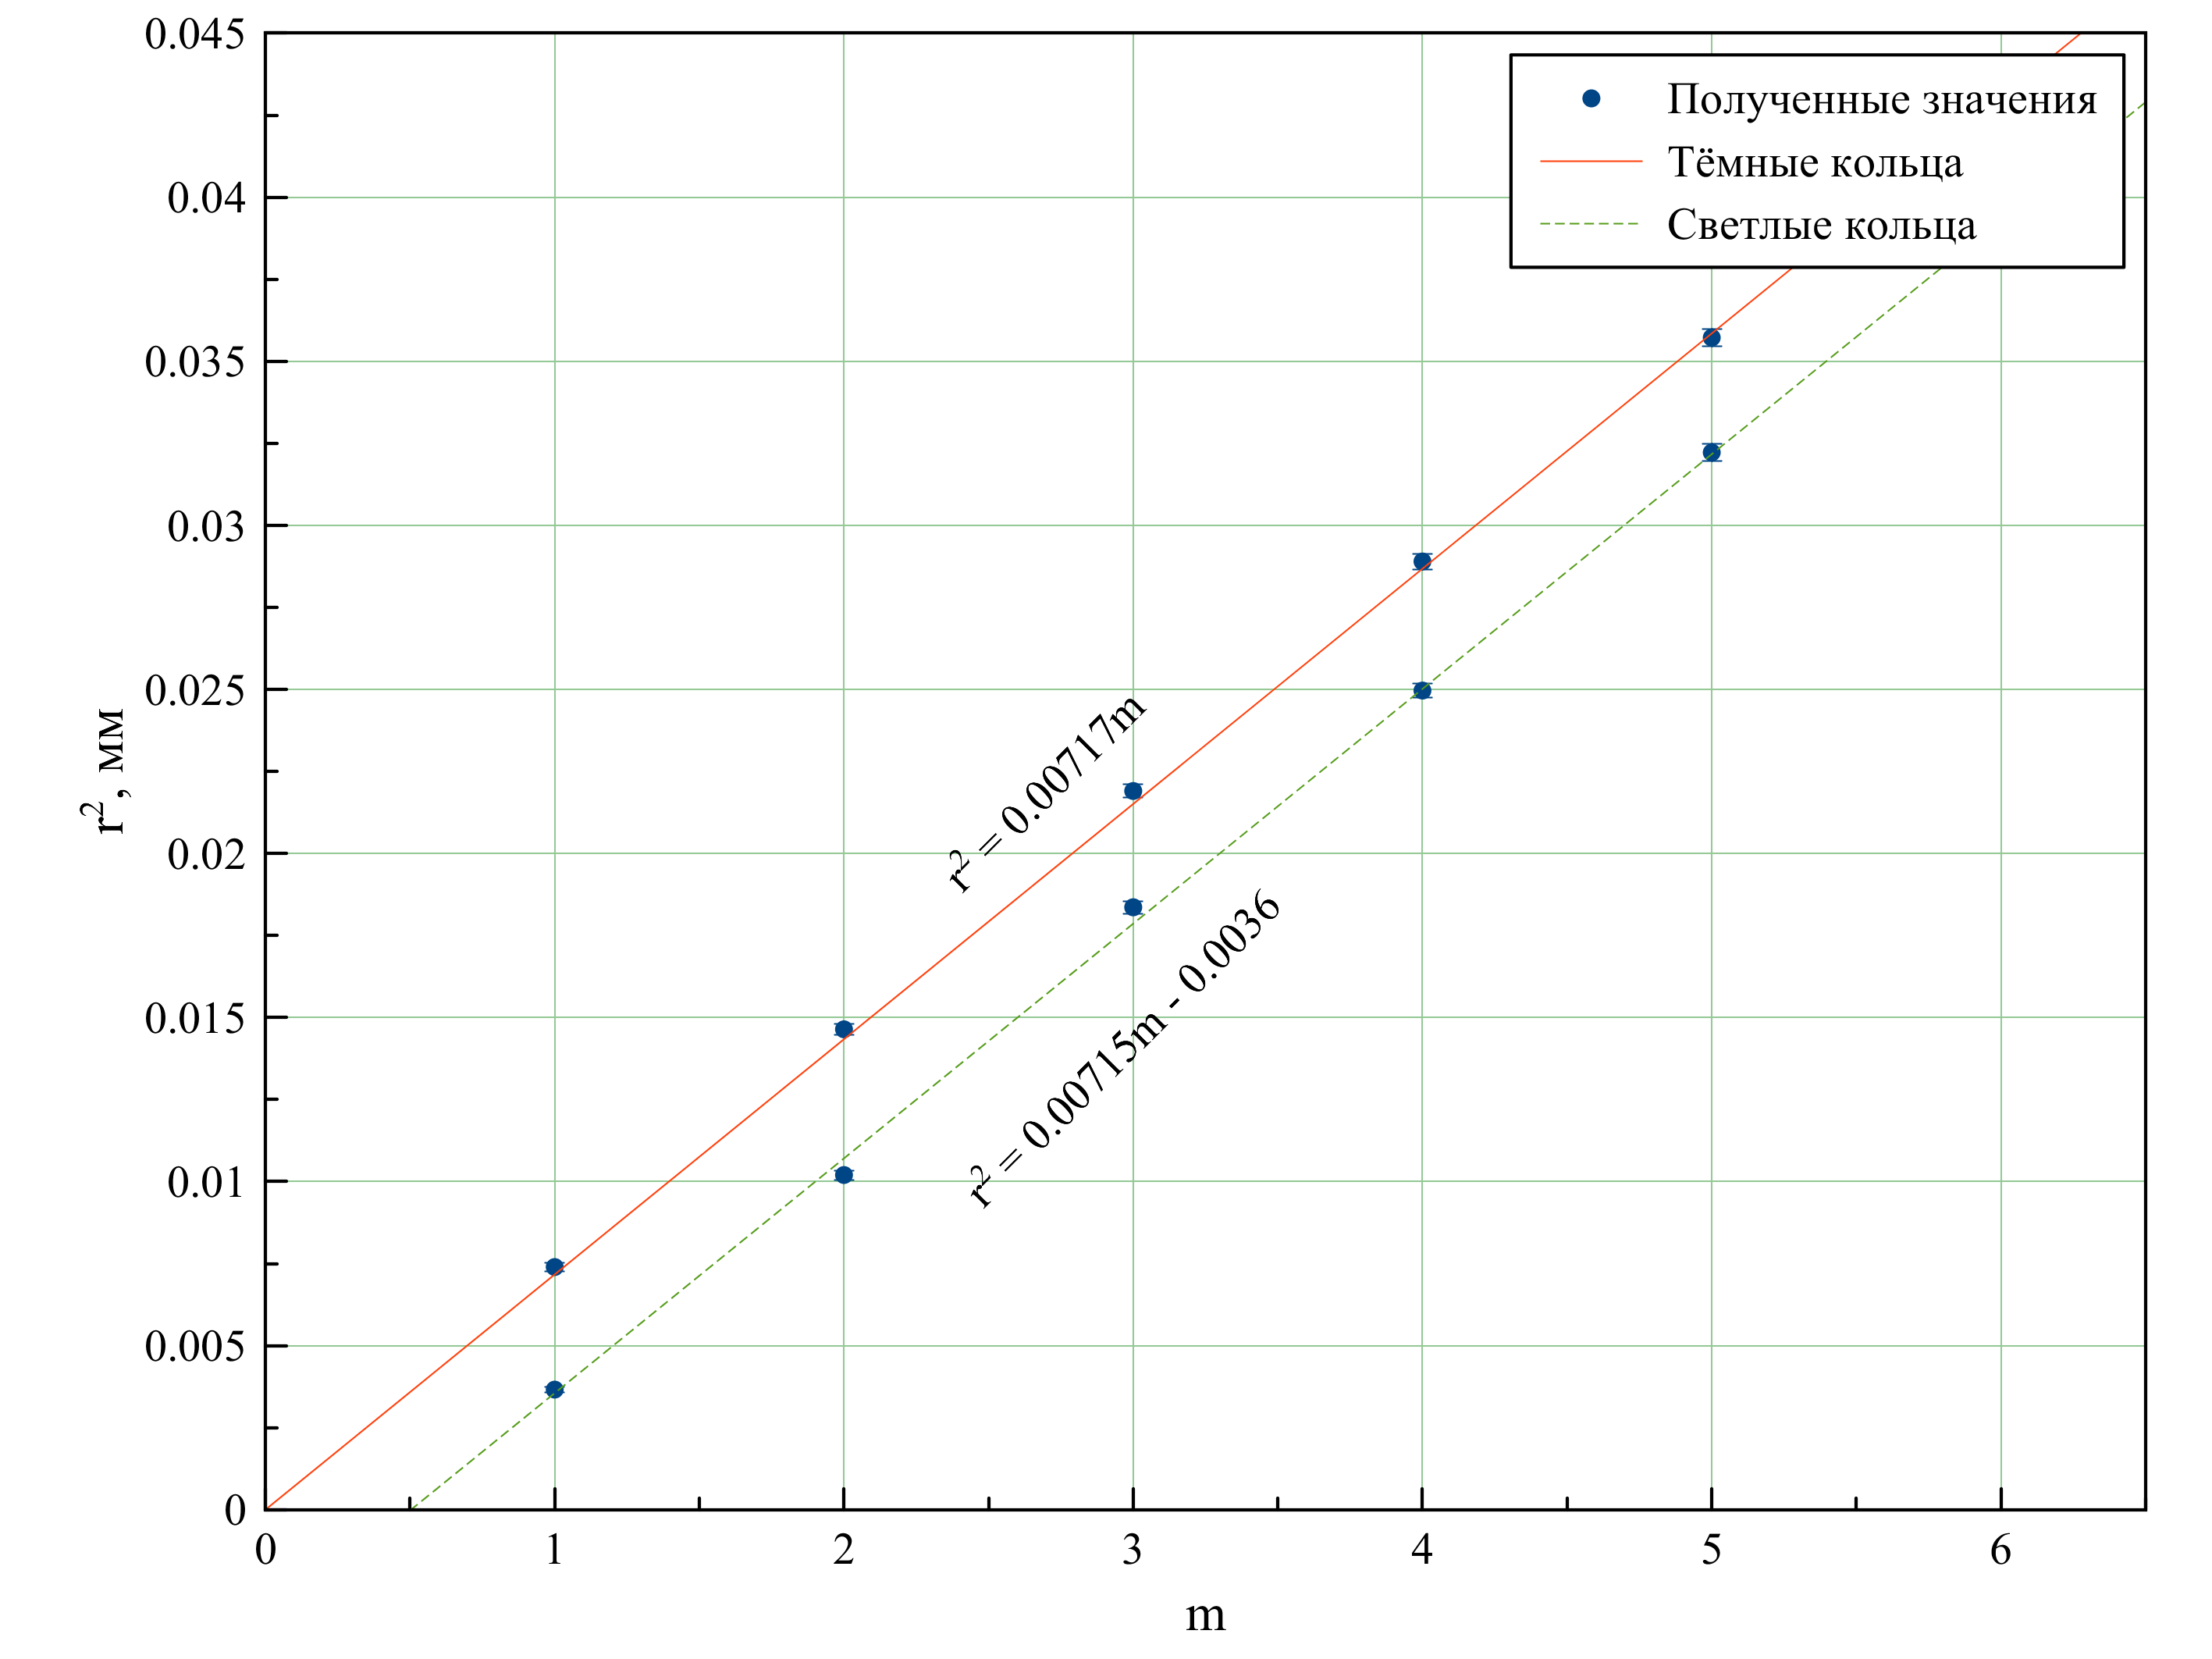
\includegraphics[width = \textwidth]{graph1}
			\caption{Зависимость $r^2$ и $(r')^2$ от m.}
			\label{graph1}
		\end{figure}
	
	График для тёмных колец проходит через начало координат. Также оценим размер тёмного пятна:
	$$d_\text{пятно} \simeq 37.5~\text{мкм}.$$
	
	\item  С помощью метода наименьших квадратов определим коэффициент наклона прямых. Получаем, что для тёмных колец $$k' = \dfrac{<r'^2\cdot m>}{<m^2>} \simeq (7.17 \pm 0.03)\cdot 10^{-3} ~\text{мм}^2$$.
	
	Отсюда, из формулы \eqref{eq1} имеем: $R = \dfrac{r'^2}{m} \cdot \dfrac{1}{\lambda} = \dfrac{k'}{\lambda}$
	
	\begin{center}
		$\fbox{$R = (13.1 \pm 0.1)~\text{мм}$}$
	\end{center}


\end{enumerate} 

\section{Вывод.}

\begin{itemize}
	\item В результате данной лабораторной работы были получены кольца Ньютона, как результат интерференции света.
	
	\item С их помощью мы определили радиус кривизны линзы, относительная погрешность примерно равна 1\%.
	
	\item Также было изучено явление <<биений>>. С его помощью мы измерили разность длин волн жёлтой и зелёной линий спектра ртутной лампы. Величина совпала с табличной.
\end{itemize}



	
	
	
\end{document}